\section{Itération2: nouveau BS englobant TCP serveur}
    \subsection{Spec}
    
    Cette partie repose sur la modification des exigences et la nouvelle Conception
        \subsubsection{L'évolution des exigences}
       
            Après avoir fait l’évaluation des résultats de performance 
            de la 1ere itération du projet, on a redéfinit les spécifications du projet. 
            Le tableau suivant montre la différence des exigences entre les deux itérations:
            \\
            \begin{table}[h!]
            \centering
            \begin{tabular}{|p{3cm}|p{3cm}|p{4cm}|p{5cm}|}
                \hline
                \multicolumn{4}{|c|}{Les changements des exigences } \\
                \hline   & Itération1 & Itération2 & Avantage de cette évolution\\
                \hline
                Protocol de communication & MQTT & TCP avec le support de MQTT &
                Moins coûteux par rapport aux paquets échangés, tout en gardant 
                la possibilité de connecter le boîtier à un serveur MQTT \\
                \hline
                Architecture du BS  &  Un cluster de brokers MQTT avec des 
                subscribers des tracks et publishers d’events.  & Un cluster de 
                TCP serveur qui gèrent les connexions, traitent les message échangés 
                et envoient/re\c coivent les msg à/de kafka. & Moins coûteux par 
                rapport aux instances à gérer. 
                Plus facile à gérer un seul composant au BS. 
                Pas de complexité à dispatcher les subscribers quand on monte de charge.\\
                \hline 
            \end{tabular}
            \caption{Tableau de comparaison des exigences du projet}
            \label{table:1}
        \end{table} \\
        La spécification téchnique peut être divisée en deux parties:
        \begin{itemize}
            \renewcommand{\labelitemi}{$\bullet$}
            \item La spec technique du protocole
            \item La spec ajoutée par \gls{mdi} pour adapter le protocole au besoin
        \end{itemize}
        \bigskip
        L’une des majeurs modifications est d'abandonner l’intégration du standard MQTT 
        tel qu il est . On ne garde que le Header de MQTT comme le Header des messages 
        échangés avec le nouveau tcp serveur. Ceci a pour but de garder la compatibilité 
        avec MQTT pour satisfaire les besoins commerciaux. 

        \subsubsection{Architecture de l'itération 2 }
            L’architecture du nouveau BS est conçue d’une façon à ce qu il présente 
            une solution aux problèmes rencontrés par l’architecture de la 1ere itération. 
            La figure ci dessous montre les composants de la nouvelle architecture:  \\
            \begin{figure}[ht]
                \centering
                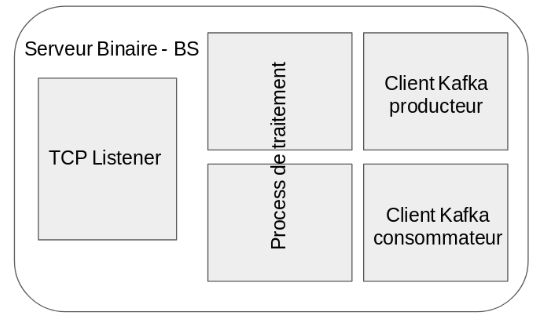
\includegraphics[scale=0.8]{\images/architecture_BS_iteration2.png}
                \caption{La conception de l'architecture du BS de l'itération 2}
                \label{Figure }
            \end{figure}
        
       
            Le BS  repose sur 3 grands composants: 
            En premier temps, le TCP serveur qui gère la connexion avec le boitier. 
            En deuxième temps,le traitement des données doit être gérer en parallèle. 
            Ce traitement assure l’encodage du protobuf boitier au protobuf cloud et 
            vis-versa. 
            D’autre part, deux clients kafka, un producteur qui va publier les messages 
            encodés et un autre consommateur qui va recevoir les messages d event. 

            \subsection{Implémentation}
            Le nouveau BS lance les diverses traitements dans des traitements en 
            parallèle. L’implémentation de ces processus parallèles s’effectuent grâce 
            aux goroutines du langage go, ce qui englobe toutes les fonctionnalités du BS 
            dans un même composant unifié.

            \subsubsection{Control plane}
             Concernant le flux de données ou Control plane, la communication entre 
             ces processus se fait comme le présente la figure ci-dessous: \\

             \begin{figure}[ht]
                \centering
                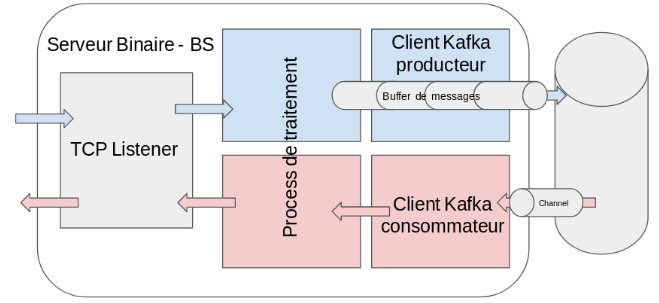
\includegraphics[scale=0.8]{\images/control_plane.png}
                \caption{Le flux de données du BS de l'itération 2}
                \label{Figure }
            \end{figure}


            * Le boitier envoie un track pour le cloud: 


            La première connexion se fait avec le TCP Listener. 
            Comme son nom l’indique, ce composant écoute, vérifie et  maintient la 
            connexion avec les boîtiers. Il est considéré comme le Générateur. 
            Après avoir vérifier la connexion avec un boitier donné, il envoie le 
            message reçu au processus de traitement dans un channel. \\
            Ce dernier décode le format du message et l’encode en format des données du 
            cloud. Ensuite il le met dans un buffer des messages prêts à la publication 
            kafka. Puis le client kafka envoie tous les messages du buffer d’une manière 
            périodique de quelques secondes.\\ 
            L’envoi des messages d’une manière périodique minimise l'accès 
            écriture dans la BD ce qui augmente l’efficacité du traitement global. 

            *  Le cloud envoie un event au boîtier: 
            Le service qui a déclenché l’event va publier dans le broker des messages le 
            message dans un topic spécifique. Le client consommateur est toujours en écoute sur ce topic, 
            il reçoit le message et l'envoie directement au traitement. Le message s’encode avec le format 
            protobuf du boitier est maintenant prêt à être envoyer au boîtier. Le TCP listener s’occupe alors 
            de son envoi à son boitier. \\
            Il est à noter que l'implémentation de cet envoi par rapport à plusieurs 
            instances sera plus complexe. 

        
       

        \subsubsection{Go un language différent}
       
        Paragraphe sur le language Go : 
        Go est un jeune language de programmation système
        fascinant. Ce language compilé hérite des idées des paradigmes de
        programmation impérative et fonctionnelle. Il définit des concepts et
        des règles qui assurent à l'utilisateur des binaires .\\[0.3cm]
       
      
        Le but de cette explication est de montrer la différence considérable
        avec d'autres langages de programmation. Un lecteur intéressé pourra
        apprendre le langage pour plus d'informations.

        {Avantages}
            \begin{itemize}
                \renewcommand{\labelitemi}{$\bullet$}
                \item basé sur les librairies basiques
                \item développé par Google donc un bon support 
                \item Evolution du language
            \end{itemize}

        {Inconvénients}
            \begin{itemize}
                \renewcommand{\labelitemi}{$\bullet$}
                \item 
                \item Pas de programmation orientée objets ou support pas standard
            \end{itemize}

    \subsection{Test }
        Apprendre Go était une très belle expérience. La réference principale
        pour moi était .... 
       ... m'a servi de réference pour
        comprendre des concepts sur le fonctionnement interne du language.
     Mais ça m'a aidé à
        comprendre un certain nombre de problèmes auquels j'ai fait face, notament:
        \begin{itemize}
            \renewcommand{\labelitemi}{$\bullet$}
            \item La notion de variance de structures\cite{variance_wiki}.
            \item Les erreurs de lifetimes
            \item Coercions de types
            \item Le unwind de threads
            \item Les phantom data
            \item Drop et l'utilisation de \textbf{Option} dans des cas spéciaux
        \end{itemize}
        \bigskip
        Il faut aussi dire que le bagage fourni par le cours de compilation à
        \establishment{} était d'une utilité exceptionnelle, surtout que
        programmer en Go, \\[0.3cm]
        Mais la piste principale pour l'apprentissage reste la pratique. Et avec
        le projet \gls{md30} j'ai eu la chance de faire des fautes, réitérer,
        apprendre des concepts et des patterns, et corriger, dans un cycle qui a
        duré 5 mois. 

    \subsection{Amélioration à effectuer}
        Data plane .. 
        